\chapter{深度学习和深度估计概述}
\section{引言}
深度学习作为机器学习的分支,近年来成为众多学者的研究热点,极大地推动了
人工智能,高性能计算,生物医学工程等关键技术的发展。
在计算机视觉,自然语言处理
等任务上带来了革命性的创新和提高。时至今日,各种深度学习算法仍然
层出不穷,不断地刷新着包括深度估计在内的众多计算机任务的各项指标。
本文使用深度学习算法来解决单目深度估计问题,故本章重点描述
深度学习理论和深度估计概述。
\section{深度学习概述}
2012年神经网络在图像识别任务竞赛上达到了超过人类的
优越表现,从此深度学习算法开始繁荣起来,学者们纷纷
展开了深度学习在各自领域的研究。本文算法和框架
主要基于深度学习算法,所以本章围绕深度学习算法对该领域
进行简要介绍。

深度学习是机器学习方法的一部分,它基于人工神经网络和表征学习。
学习可以是有监督的、半监督的或无监督的。
大量的研究和实验证明,每个算法和每个系统最终都
可以表示为一个数学函数或一个集合到另一集合的映射,
神经网络可以很好地去拟合任何一种映射,
在大数据和算力的支撑下,
这种使用数据和算力去拟合映射的方法十分有效。
神经网络就像人脑一样,由神经元组成。
每个神经元接收信号作为输入,将其乘以权重,
求和并应用非线性函数计算最后输出结果。这些神经元是堆叠在一起,
并组织成层,最终组织成网络。

神经网络能够使用大量的数据和反向传播迭代算法来学习期望的函数。
通过向网络提供数据,通过计算图最终计算产生一个输出,
使用损失函数对输出与期望的输出进行比较,然后根据差异重新调整权重。
权值的调整是使用梯度下降的非线性优化算法来执行的。
经过一段时间的训练,由于中间层的权重
被逐步优化,网络产生的输出将会十分接近期望输出。
这时如果把一个没有被送入过网络的输入给网络,它会根据
学习好的权重计算出一个接近真实标注的输出。
\begin{figure}
    \centering
    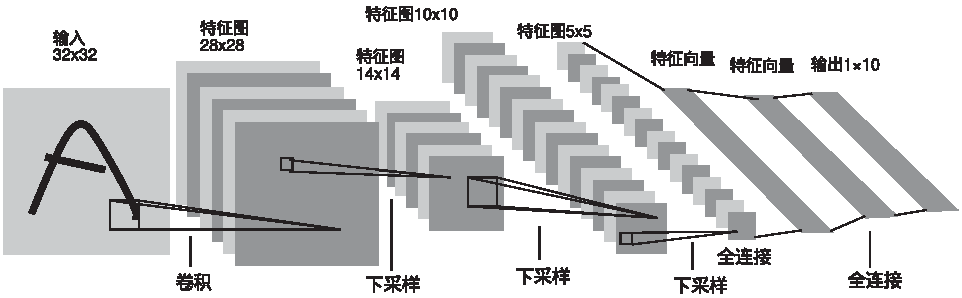
\includegraphics[scale=0.9]{figure/Lenet.pdf}
    \caption{LeNet\cite{lenet}卷积神经网络示意图}
    \label{lenet}
\end{figure}
\section{深度学习基础}
深度学习算法提出以来不断优化创新,依赖着数据,算力,网络结构的发展
在诸多领域取得了领先的效果。卷积神经网络(CNN),循环神经网络
(RNN),对抗生成网络(GAN),图卷积网络(GCN)等各种神经网络
逐渐涌现出来。由于算法主要使用了卷积神经网络,故本节对
卷积神经网络进行简要介绍。
\begin{algorithm}[htb]
	\KwIn{$m$个训练样本}
	\lFor{$l=1$ \emph{\KwTo} $n_l$}{
		初始化:$\Delta \bm{W}^{(l)}=0$,$\Delta \bm{b}^{(l)}=0$}
	\ForEach{训练样本}{
		\lFor{$l=1$ \emph{\KwTo} $n_l-1$}{
			前向传播:$\bm{z}^{(l+1)}=\bm{W}^la^l+\bm{b}^l$,$\bm{a}^{(l+1)}=f(\bm{z}^{(l+1)})$}
		输出误差计算:$\delta^{(n_l)} = \frac{\partial}{\partial \bm{z}^{(n_l)}} J(\bm{W},\bm{b};\bm{x},y)$\;
		\lFor{$l=n_l-1$ \emph{\KwTo} $1$}{
			后向传播:$\delta^{(l)} = \bigl((\bm{W}^{(l)})^T \delta^{(l+1)}\bigr)f'(\bm{z}^{(l)})$}
		\ForAll{层l}{
			计算梯度:$\nabla_{\bm{W}^{(l)}}J(\bm{W},\bm{b};\bm{x},y)=\delta^{(l+1)}(\bm{a}^{(l)})^T$ \\
			\hspace{60pt}$\nabla_{\bm{b}^{(l)}}J(\bm{W},\bm{b};\bm{x},y)=\delta^{(l+1)}$\;
			累加梯度:$\Delta \bm{W}^{(l)} \leftarrow \Delta \bm{W}^{(l)} + \nabla_{\bm{W}^{(l)}}J(\bm{W},\bm{b};\bm{x},y)$; \\
			\hspace{60pt}$\Delta \bm{b}^{(l)} \leftarrow \Delta \bm{b}^{(l)} + \nabla_{\bm{b}^{(l)}}J(\bm{W},\bm{b};\bm{x},y)$\;
		}
	}
	\ForAll{层$l$}{
		更新权重:$\bm{W}^{(l)} \leftarrow \bm{W}^{(l)} - \alpha \biggl[\frac 1m \Delta \bm{W}^{(l)}\biggl]$ \\
		\hspace{60pt} $\bm{b}^{(l)} \leftarrow \bm{b}^{(l)} - \alpha \biggl[\frac 1m \Delta \bm{b}^{(l)}\biggr]$
	}
	\caption{梯度下降与反向传播算法}
	\label{sgd}
\end{algorithm}

卷积神经网络示意图如图\ref{lenet}所示,
它由多层感知层构成,这些感知层可以提取数据
的多元抽象特征,利用这些特征的加权计算
完成对输入到输出的各种映射。
深度学习算法的步骤可以分为:
\begin{enumerate}
	\item 初始化权重计算。神经网络初始化权重,进行前向传播,计算图从前向后
	计算。
	\item 计算损失函数。最终输出与真实标注通过损失函数进行距离计算,衡量
	预测与标签之间的误差。
	\item 计算梯度,更新权重。即反向传播过程,利用优化算法更新神经网络
	中的权重,拉近输出于标签之间的距离。
	\item 循环迭代。不断重复上述过程,更新神经网络权重,直至结果达到预期。
\end{enumerate}

\section{双目深度估计基础}
双目深度估计(Binocular Depth Estimation)
也称作双目立体匹配(Stereo Matching)。有成本低,速度快等优点,立体匹配是立体视觉和
三维重建研究中的关键部分。
\begin{figure}
    \centering
    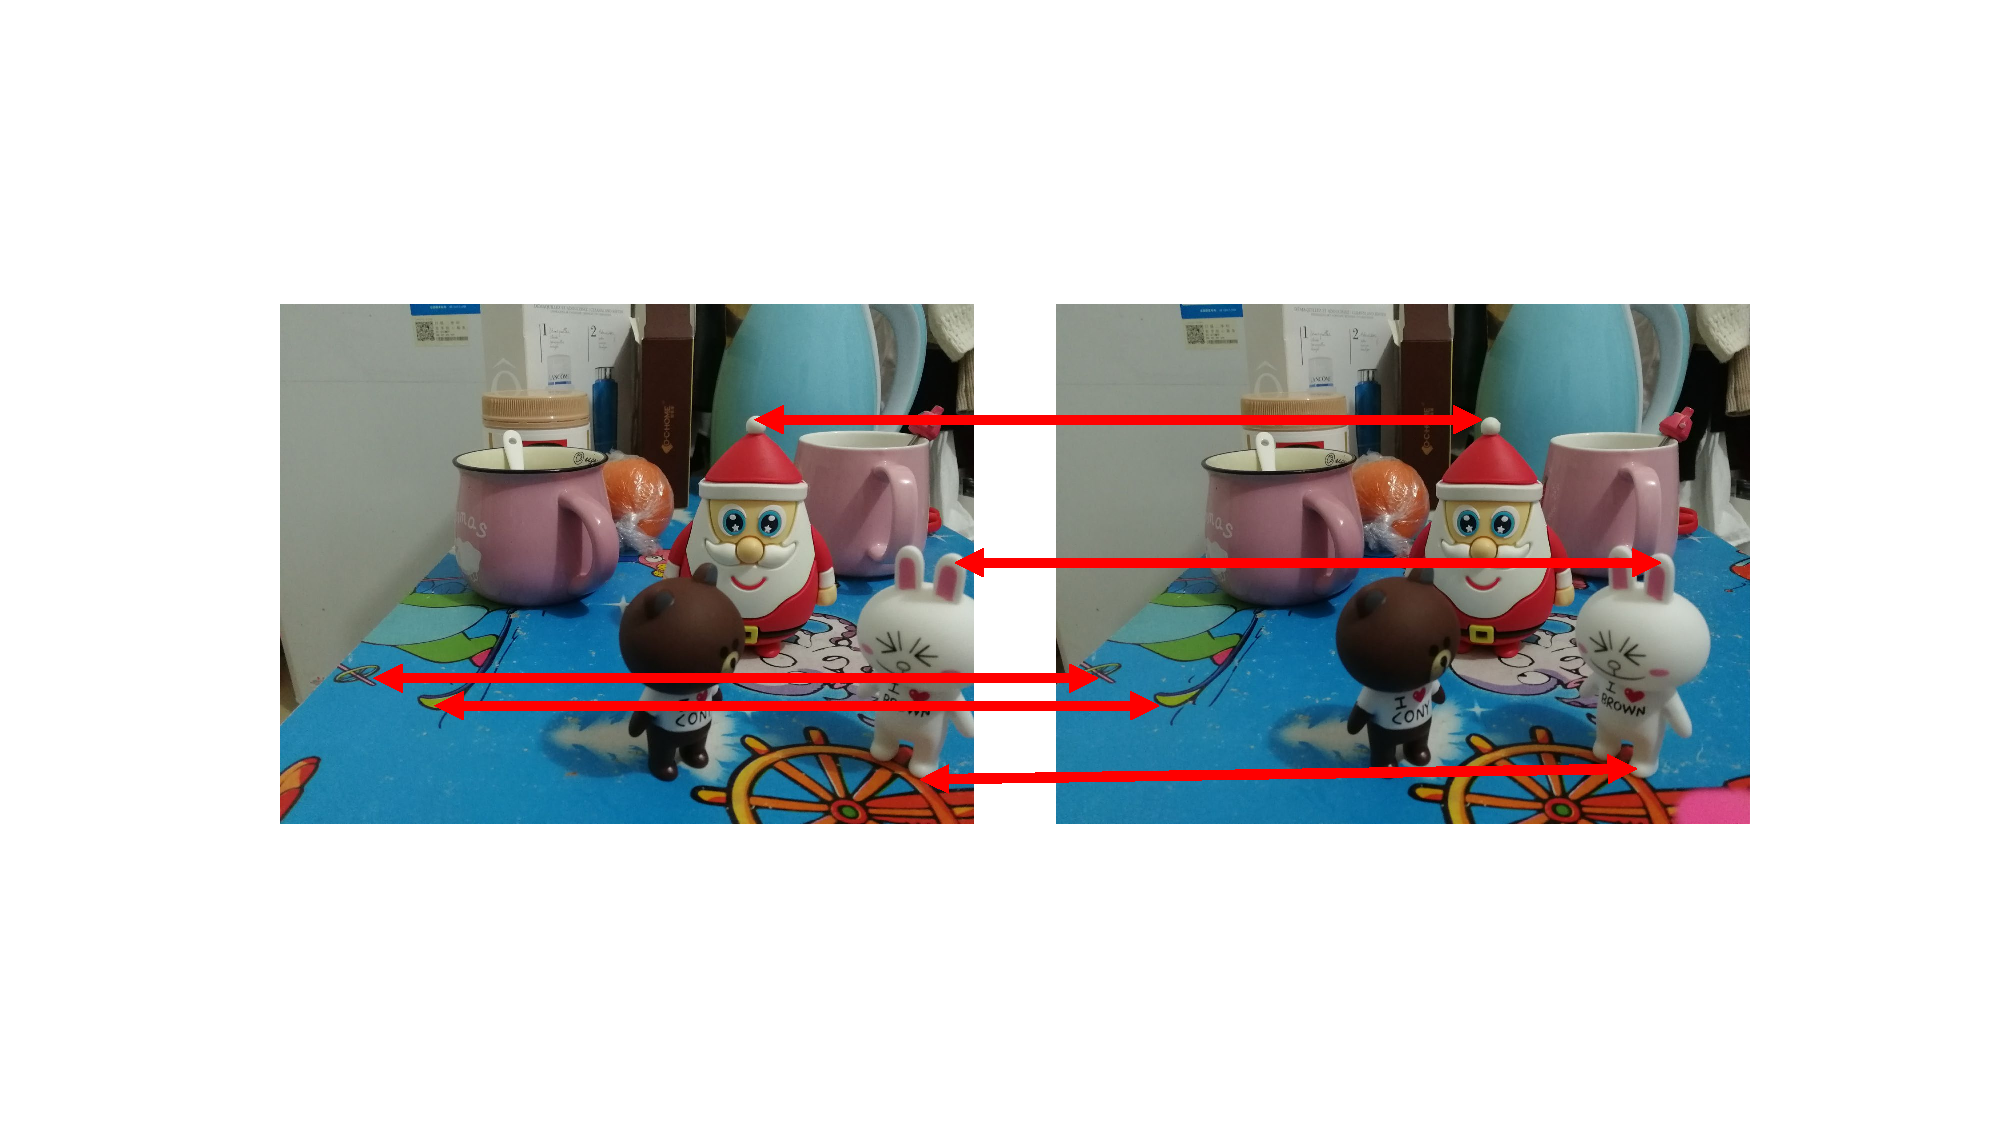
\includegraphics[width=0.8\linewidth]{figure/stereo_match.pdf}
    \caption{双目立体匹配}
    \label{stereo}
\end{figure}
其输入是一对在同一时刻捕捉到的,经过极线校正的左右图像$I_l$和$I_r$。
而它的输出是由参考图像(一般以左图作为参考图像)中每个像素对应的视差
值所构成的视差图$d$。视差是三维场景中某一点在左右图像中对应点位置的像
素级差距。当给定摄像机的基线距离$b$和焦距$f$之后,就可
以从视差图中自动计算出深度:$D = bf/d$,所以深度和视差是可以互相转换,
相互等价的。
立体匹配算法一般分为四个步骤:
\begin{enumerate}
	\item 匹配代价计算(Matching Cost Computation)
	\item 代价聚合(Cost Aggregation)
	\item 视差计算(Disparity Computation)
	\item 视差精修(Disparity Refinement)
\end{enumerate}

\subsection{双目深度估计原理}
其目标是在两个或多个视点中匹配相应像素点,计算视差,
并通过对能量代价函数最小化来估计像素点的视差,求得深度。
这是一个从二维信息中恢复三维信息的过程。
原理图如图\ref{stereo matching}所示:
\begin{figure}[ht]
 \centering
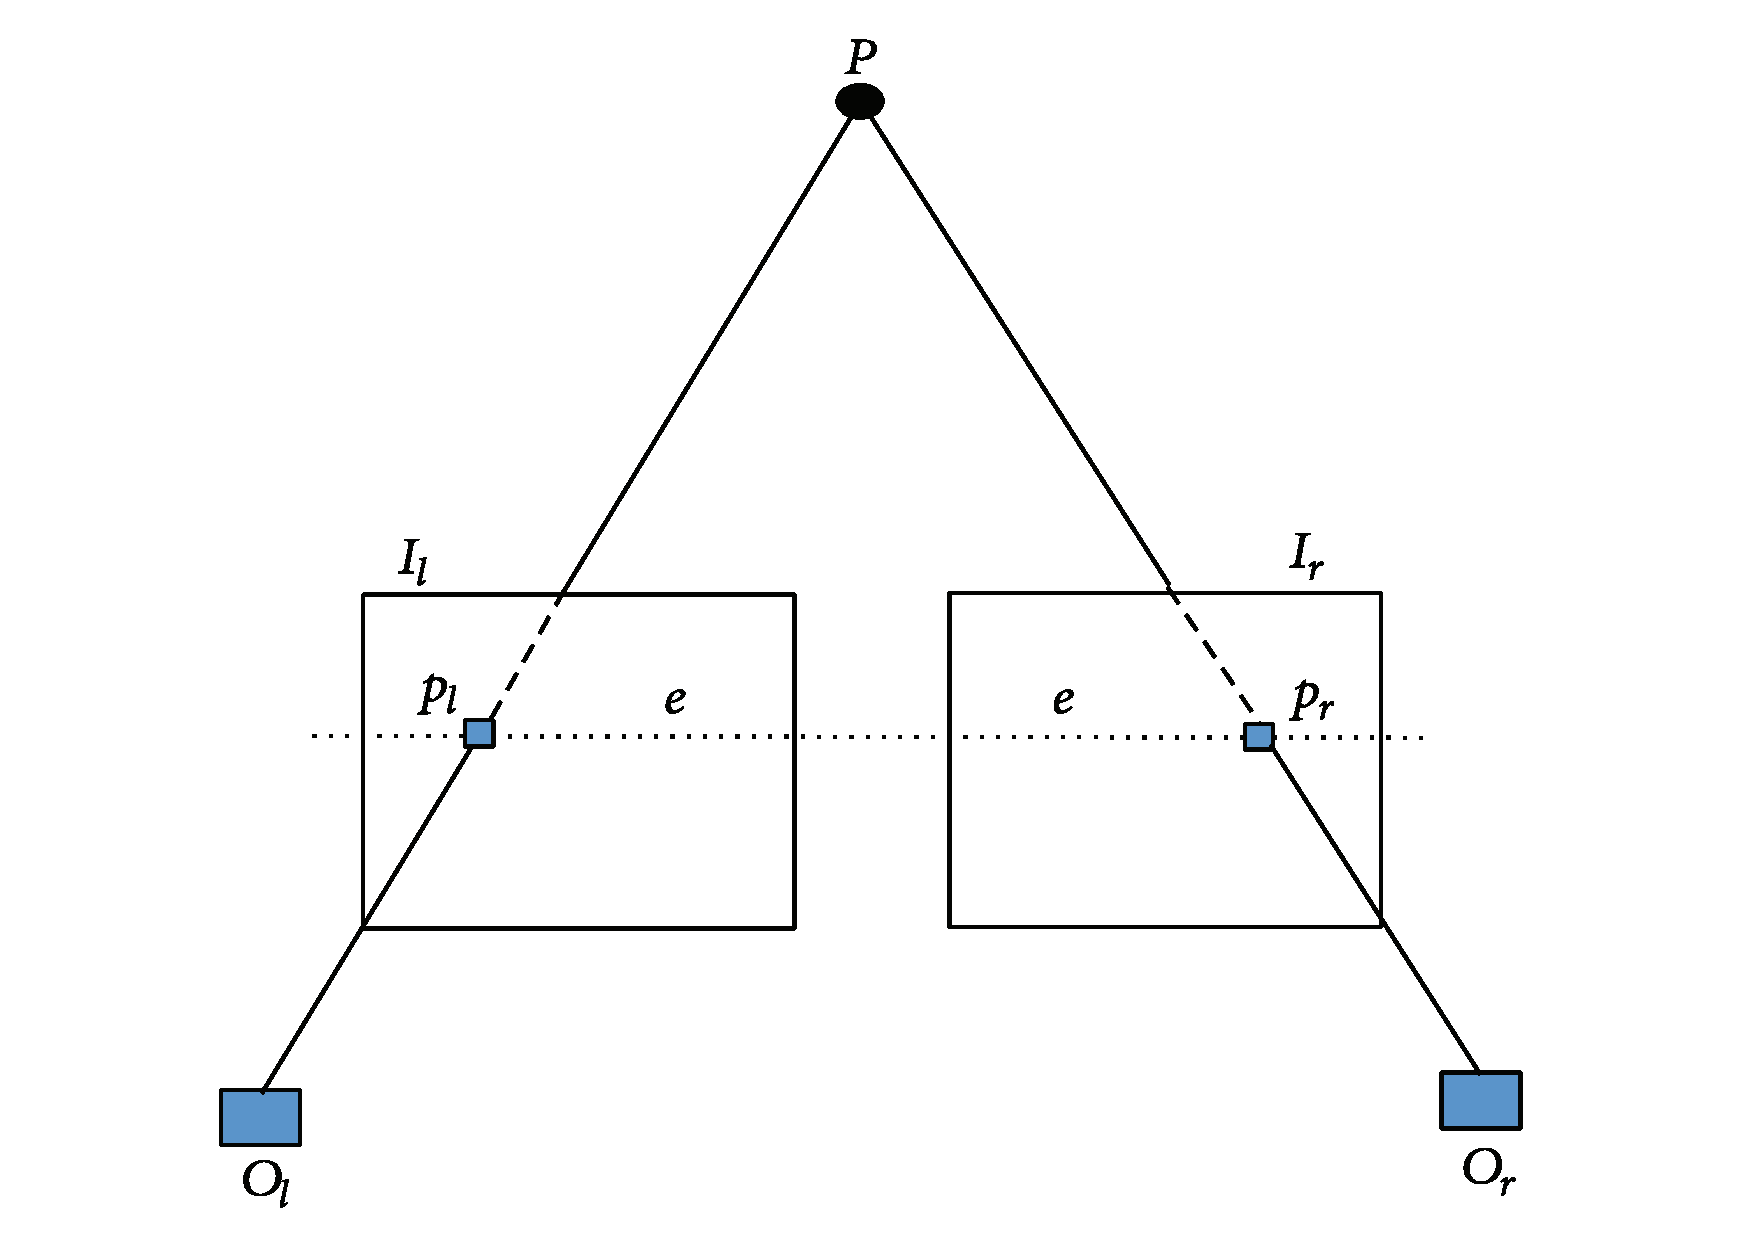
\includegraphics[width=0.5\linewidth]{figure/stereo_theory.pdf}
\caption{立体匹配获得视差,进而获得深度信息}
\label{stereo matching}
\end{figure}
上图中所在位置为Projector光源所在位置,
$o_l$所在位置为左相机光心,
$o_r$所在位置为右相机光心,$I_l$与$I_r$
分别为左成像面与右成像面。$p_l$与$p_r$分别为
光源\emph{P}在成像面上的位置。
根据成像原理$o,p_l,p$共线,$o,p_r,p$共线。
根据相似三角形原理,在特征点已经匹配的基础上,
可以计算出特征点的深度信息。
然而,特征点的匹配并不是一件非常简单的事情,
场景中的纹理,光照,透明,反光等情况均会影响匹配结果。
尤其是纯双目视觉中特征点的匹配,涉及到非常复杂的计算过程。

\subsection{双目估计常用数据集}
\subsubsection{KITTI}
\label{kitti}
KITTI数据集是一个计算机视觉领域常用数据集,其具体适用任务有很多,
例如光流估计,视觉里程估计,深度估计,物体检测,语义分割,
物体跟踪等子任务。它由装备在一台汽车上的传感器来进行采集,采集到的
信息包括双目彩色视频,双目黑白视频,雷达点云信息,惯性导航信息,
GPS信息等。原始数据量十分庞大。每个场景都包含一对双目RGB
图像和对应的深度信息,分辨率为$1224 \times 368$。因为
数据集包含真实标注和立体双目图像,所以它既适用于监督方法也适用于
无监督或者半监督方法。在使用上,KITTI有两种不同的划分。
其中在Eigen Split选取了61个场景中的28个作为测试场景,
从中选出了697张图像用来测试。在另外的28个场景中选出
了26000张图像用于训练。而 KITTI split 包含29,000张训练图像,
200张测试图像。另外,由于没有官方的稠密深度图,不同论文会对
稀疏点云进行不同的预处理。
\subsubsection{Middlebury}
Middlebury\cite{middlebury}为双目深度领域常用的数据集。分为
五次公开,2001年公开6个子集,2003年公开2个,2005年公开
9个,2006年公开21个,2014年公开33个。现在Middlebury已经发展为
主流的测试数据集之一。
\subsubsection{Sceneflow}
Sceneflow数据集是一个虚拟合成数据集,由德国弗莱堡大学与
慕尼黑大学一起整理构建。数据集包含三个子集,分别是虚拟道路数据集
Driving,含有4392对双目图像;虚拟场景数据集FlyingThings3D,由
21818对训练和4248对测试双目图像构成;动画场景数据集Monka,由
8591对双目图像构成。图片分辨率均为$540 \times 960$。
\subsection{评价体系}
双目立体匹配常采用均方根误差(Root Mean Squared Error, RMSE)
以及匹配错误像素所占百分比来
作为评价标准。
1. RMSE(Root Mean Squared Error)是衡量预测视差$d_p(x,y)$与
真实视差$d_g(x,y)$的指标:
\begin{align}
	RMSE = \sqrt{\frac{1}{N}\sum_{(x,y)}|d_p(x,y)-d_g(x,y)|^2}
\end{align}
2. 错误匹配所占百分比:
\begin{align}
	B = \frac{1}{N}\sum_{(x,y)}|d_p(x,y)-d_g(x,y)| > \delta
\end{align}
其中$\delta$代表对匹配错误像素的容忍度。
%\subsection{表格举例}
%表 \ref{tab1} 表示……。
%\begin{table}[h]
%	\centering
%	\caption{国际单位制中具有专门名称的导出单位}		
%	\label{tab1}
%	\begin{tabular}{c|c|c|c}
%		\toprule[2pt]
%		量的名称 & 单位名称 & 单位符号 & 其他表示式例\\
%		\midrule[2pt]
%		频率	& 赫[兹]	& Hz	&$s^{-1}$ \\
%		\hline                                        %细横线
%		力;重力 	& 牛[顿]	& $N$	 & $kg·m/s^2$ \\
%		\hline                                         %细横线
%		压力,压强;应力	& 帕[斯卡]	&$Pa$	&$N/m^2$ \\
%		\bottomrule[2pt]
%	\end{tabular}
%\end{table}
%
%\subsection{公式举例}
%\label{sec:formula}
%没有编号的公式:
%\begin{equation*}
%\bm{z}^{(l)} = \bm{W}^{(l)}\bm{a}^{(l-1)} + \bm{b}^{(l)} 
%\end{equation*}
%
%公式中含有中文:
%\begin{equation}
%\mbox{像素准确率} = \sum_{i=1}^{n_{cl}}n_{ii} / \sum_{i=1}^{n_{cl}}t_i
%\end{equation}
%
%公式中含有矩阵:
%\begin{equation}
%\label{eq1}
%\textbf{H} = \begin{bmatrix}
%I*\bm{x}_i \\ \textbf{h}
%\end{bmatrix}
%\end{equation}
%
%多行公式:
%\begin{align} 
%\hat{\bm{R}}_r 
%& =   \frac{1}{N_s} \sum_{i=1}^{Ns} \bm{r}_i \bm{r}_i^T  \label{Eq-2-a} \\
%& =   \frac{1}{N_s} \sum_{i=1}^{Ns} \bm{r}_i \bm{r}_i^T  \nonumber \\
%& =   \frac{1}{N_s} \sum_{i=1}^{Ns} \bm{r}_i \bm{r}_i^T  \label{Eq-2-c},
%\end{align}
%
%引用:公式 \eqref{eq1} ……,\eqref{Eq-2-a}……。
%
%更多的数学公式编辑方法,请参考根文件下“LaTex学习文档”中的文献1和文献3。
%
%\subsection{算法举例}
%
%
%
%算法 \ref{sgd}……。
%
%\subsection{例子}
%\begin{eg}
%	这是一个例子。
%	\label{eg1}
%\end{eg}
%例 \ref{eg1} ……。
%
%\subsection{证明}
%\begin{proof}
%证明过程
%\end{proof}
%
%\subsection{定理}
%\begin{theorem}
%	这是一个定理。
%	\label{th1}
%\end{theorem}
%定理 \ref{th1} ……。
%
%\subsection{命题}
%\begin{proposition}
%	这是一个命题。
%	\label{pro1}
%\end{proposition}
%命题 \ref{pro1} ……。
%
%\subsection{引理}
%\begin{lemma}
%	这是一个引理。
%	\label{lem1}
%\end{lemma}
%引理 \ref{lem1} ……。
%
%\subsection{推论}
%\begin{corollary}
%	这是一个推论。
%	\label{cor1}
%\end{corollary}
%推论 \ref{cor1} ……。
%
%\subsection{定义}
%\begin{definition}
%	这是一个定义。
%	\label{def1}
%\end{definition}
%定义 \ref{def1} ……。
%
%\subsection{标记}
%\begin{remark}
%	这是一个标记。
%	\label{rem1}
%\end{remark}
%标记 \ref{rem1} ……。
\section{单目深度估计基础}

\subsection{单目估计常用数据集}
深度学习算法需要大量的数据来给神经网络“学习”,
强大的算力使神经网络去学习数据的分布。所以每个
视觉任务下都出现了大量的数据集。
例如手写字符数据集MNIST\cite{lecun2010mnist},识别数据集
CIFAR-10\cite{Krizhevsky}和CIFAR-100\cite{Krizhevsky}。
还有一些针对多种任务构建的大型数据集,
例如ImageNet\cite{imagenet}包含分类,物体检测,和语义分割等任务,
MS-COCO\cite{coco}包含物体检测,语义分割和图片描述任务。
单目深度预测任务下常用的数据集有KITTI\cite{kitti},
NYU depth\cite{nyu},Make 3D\cite{Make3D},
Scannet\cite{scannet},以及Cityscapes\cite{cityscapes}。
本小节对这些数据集进行了
简介和梳理。值得一提的是,有些双目深度估计数据集也可以用在单目深度估计任务上。

\subsubsection{KITTI}
由于KITTI数据集有双目图像,和真实深度标注,
所以单、双目深度估计方法
都可以采用KITTI进行训练,KITTI已在\ref{kitti}介绍。

\subsubsection{NYU depth}
NYU depth数据集是常用的深度估计数据集,它主要关注室内环境,
数据集由464个室内场景组成,
其中249个场景用作训练,215个场景用作测试。不同于KITTI数据集
使用激光雷达来采集深度信息,NYU depth数据集使用
Microsoft的Kinect RGB-D相机来采集视频序列和对应的深度。
图像和深度图的分辨率为$480 \times 640$,通常会在实验中
下采样减半来加速训练过程。为了去掉冗余的边缘信息,
还会将图像进行中心裁剪到$228 \times 304$。
因为不同的RGB相机和深度相机之间
不是完全同步的,深度图和RGB图像之间不是一对一的对应关系。
为了对齐深度图和RGB图像,每个深度图都与最近的RGB图像同步并且
关联在一起。由于硬件原因,采集到的深度图通常会有空洞,
这些空洞可以
使用数据集提供的工具箱进行填补,具体地预处理方法并不是统一的。
\subsubsection{Make3D}
Make3D数据集仅由单目RGB图像以及深度图像组成,
不同于上述数据集的图像。由于没有双目图像或者
视频序列,该数据集只能用于有监督训练。它被广泛用作
评估无监督算法的测试集。
采样工作使用定制的三维扫描仪来完成,数据集收集了534幅图像
以及对应的深度图,图像分辨率2272x1704,深度图分辨率55x305,
其中400幅用来训练,134张用来测试。
\subsubsection{ScanNet}
ScanNet相比其他数据集拥有完全的语义标注。作者构建了一个
数据采集系统来进行采样。采样工作由不同国家的
20个人手持带有深度摄像头的
ipad拍摄RGB-D视频来完成。然后在Mechanical Turk平台上有
500多名工作人员进行注释。
由于提出的框架以无人监督的方式运行,并且人们不断收集数据,
因此该数据集在持续增长。数据集包含1513个场景中的2.5M个视角,
共21个类别的对象,其中,1201个场景用于训练,312个场景用于测试,
并标注了深度信息,表面重建信息,语义信息,相机姿态信息。
\subsubsection{Cityscapes}
Cityscapes构建主要是为了推动城市语义场景理解的发展,
其本身并没有真实的深度标注。该数据集的图像是由装备在
一辆行驶中的车辆上的相机进行采集,覆盖了主要在德国及周边城市
50个城市的春、夏、秋三季的日间场景,原始数据达到了数十万帧。
处理后的数据包含5000张精细处理图像以及20000张粗放处理图像。
由于没有真实深度标注,该数据集只能是用于无监督方法,
通常使用22973对分辨率为$1024 \times 2048$的双目图像对
来进行无监督训练。或者使用该数据集进行预训练来提高网络对
室外场景的稳定性。

\subsection{评价体系}
为了客观的评价和比较不同的深度估计方法的效果,
Eigen等人\cite{eigen2014depth}提出了五个评价指标。这些指标
为后续的工作提供了一致的指标。
\begin{align}
 RMSE=\sqrt{\frac{1}{\lvert N \rvert} \sum\nolimits_{i\in N}\lvert|d_i - d_i^*\rvert|^2} 
\end{align}
\begin{align}
  RMSE \ log = \sqrt{\frac{1}{\lvert N \rvert}\sum\nolimits_{i\in N}\lvert| \lg(d_i) - \lg(d_i^*) \rvert|^2}
\end{align}
\begin{align}
  Abs \ Rel=\frac{1}{\lvert N \rvert}\sum\nolimits_{i \in N}\frac{\lvert d_i - d_i^* \rvert}{d_i^*}
\end{align}
\begin{align}
  Sq \ Rel=\frac{1}{\lvert N \rvert}\sum\nolimits_{i \in N}\frac{\lvert| d_i - d_i^* \rvert|^2}{d_i^*}
\end{align}
\begin{align}
  Accuracies:\% \ of \ d_i \ s.t. \max(\frac{d_i}{d_i^*},\frac{d_i^*}{d_i})=\delta < thr 
\end{align}
式中$d_i$ 和 $d_i^*$ 分别代表预测深度值和真实深度之. $N$ 是图像中
的有效像素综述, $thr$ 代表了三个不同的尺度:$1.25$, $1.25^2$, $1.25^3$. 
\section{本章小结}
本章重点介绍了深度估计与深度学习方面的相关技术背景,例如深度学习的发展历史,
深度学习基础,深度估计基础等。深度学习发展几经波折,经过了两次低谷
三次繁荣,最终依托数据,算力和网络结构在诸多领域取得优异的成绩。
简述了深度学习的基础流程:初始化权重,前向传播,反向传播,迭代优化和
一些基本概念。随后从深度估计的高度对单目深度估计和双目深度估计
进行梳理总结,包括其原理,方法,常用数据集,常用衡量指标等。
使没有任何基础的读者对后续方法有一些背景知识上的了解。